\section{Model Equations}   
The final model equations are presented in this section.
The model equations will be presented, linarized and put into state space.
\autoref{fig:boat3DForces} and \ref{fig:boat2D} show a diagram of the vessel.
The model equations are presented in to body frame, meaning all movement is relative to the boat. 
The states can be transformed into the inertial frame, using equation \autoref{eq:RotMatrix}.  
\begin{figure}[H]
    \captionbox  %<--use captionbox instead if no global caption is needed
    {               %                                \%-%-%-%-%-%-%\
        Diagram of the boat where the forces applied by the motors are shown.                %\
        \label{fig:boat3DForces}                                  %\
    }                                                                 %\
    {                                                                  %\
        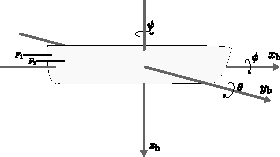
\includegraphics[width=.46\textwidth]{figures/boat3DForces}         %\
    }                                                                    %\
    \hspace{5pt}                                                          %\
    \captionbox  %<-----------------------------------------------------%\
    {       
        Above perspective of the vessel, where the distances needed for the model equations are presented.                                                                %\                         %\
        \label{fig:boat2D}                                     %\
    }                                                                           %\
    {                                                                            %\
        \includegraphics[width=.2\textwidth]{boat2D}            %|
    }                                                                             %|
\end{figure}
%
The translational movement of the vessel is described by \autoref{eq:x_pos_model}, \ref{eq:y_pos_model} and \ref{eq:z_pos_model}.
The model relates the forces applied by the motors to the boat frame. 
%
\begin{flalign}
	m_\mathrm{x} \ddot{x}_\mathrm{b} &=  F_\mathrm{1} + F_\mathrm{2}  - d_{\dot{x}_\mathrm{b}} \dot{x}_\mathrm{b} + F_{x_\mathrm{b}}
    \label{eq:x_pos_model} \\
    m_\mathrm{y} \ddot{y}_\mathrm{b} &=  -d_{\dot{y}_\mathrm{b}} \dot{y_\mathrm{b}} + F_{y_\mathrm{b}}
    \label{eq:y_pos_model} \\
    m_\mathrm{z} \ddot{z}_\mathrm{b} &=  -d_{\dot{z}_\mathrm{b}}\dot{z_\mathrm{b}} + F_{z_\mathrm{b}} \label{eq:z_pos_model}
\end{flalign}
%
\begin{where}
	\va{m_\mathrm{x,y,z}}{Is the virtual mass in their respective direction}{kg}
%    \va{m_\mathrm{x}}{}{kg}
%    \va{m_\mathrm{y}}{}{kg}
%    \va{m_\mathrm{z}}{}{kg}
    \va{\ddot{x}_\mathrm{b}}{is the acceleration in the $x_\mathrm{b}$ direction}{m s^{-2}}
    \va{\ddot{y}_\mathrm{b}}{is the acceleration in the $y_\mathrm{b}$ direction}{m s^{-2}}
    \va{\ddot{z}_\mathrm{b}}{is the acceleration in the $z_\mathrm{b}$ direction}{m s^{-2}}
    \va{\dot{x}_\mathrm{b}}{is the velocity in the $x_\mathrm{b}$ direction}{m s^{-1}}
    \va{\dot{y}_\mathrm{b}}{is the velocity in the $y_\mathrm{b}$ direction}{m s^{-1}}
    \va{\dot{z}_\mathrm{b}}{is the velocity in the $z_\mathrm{b}$ direction}{m s^{-1}}
    \va{F_1}{is the force applied by motor 1}{N}
    \va{F_2}{is the force applied by motor 2}{N}
\end{where} \\
% 
From the equations it shows that only the x-axis on the boat frame is controllable, as this is the axis containing the main thrusters. 
While the vessel do contain side thrusters, they are only intended for fine maneuvering, as their strength is relatively weak, compared to the main thrusters.\\
%
The virtual mass components is the added mass from the displaced water in the respective direction plus the mass of the vessel.
This value will be different for each axis, as the difference in shape drags a different amount of water with it depending on the direction.
    
The angular movement of the vessel is described by \autoref{eq:phi_model}, \ref{eq:theta_model} and \ref{eq:psi_model}.

\begin{flalign}
    I_\mathrm{x}\ddot{\phi} &= -d_{\dot{\phi}} \dot{\phi} + T_\mathrm{\phi}  
    \label{eq:phi_model} \\
    I_\mathrm{y}\ddot{\theta} &= -d_{\dot{\theta}} \dot{\theta} + T_\mathrm{\theta}  
    \label{eq:theta_model} \\
    I_\mathrm{z}\ddot{\psi} &= F_\mathrm{1}l_\mathrm{1} - F_\mathrm{2} l_\mathrm{2} - d_{\dot{\psi}} \dot{\psi} \label{eq:psi_model}
\end{flalign}
%
\begin{where}
    \va{I_\mathrm{x}}{is the inertia around the $x_\mathrm{b}$ axis}{kg}
    \va{I_\mathrm{y}}{is the inertia around the $y_\mathrm{b}$ axis}{kg}
    \va{I_\mathrm{z}}{is the inertia around the $z_\mathrm{b}$ axis}{kg}
    \va{\ddot{\phi}}{is the angular acceleration around the $x_\mathrm{b}$ axis}{rad s^{-2}}
    \va{\ddot{\theta}}{is the angular acceleration around the $y_\mathrm{b}$ axis}{rad s^{-2}}
    \va{\ddot{\psi}}{is the angular acceleration around the $z_\mathrm{b}$ axis}{rad s^{-2}}
    \va{\dot{\phi}}{is the angular velocity around the $x_\mathrm{b}$ axis}{rad s^{-1}}
    \va{\dot{\theta}}{is the angular velocity around the $y_\mathrm{b}$ axis}{rad s^{-1}}
    \va{\dot{\psi}}{is the angular velocity around the $z_\mathrm{b}$ axis}{rad s^{-1}}
    \va{l_1}{is the perpendicular distance from motor 1 to the center of gravity}{m}
    \va{l_2}{is the perpendicular distance from motor 2 to the center of gravity}{m}
\end{where}

Similar to the translatoric equations, only one axis is controllable, due to the lack of actuators. 
This will not be a problem in practice, as yaw is the only direction that it desirable to control, and any torque induced upon the other axis is a be product of the dynamics.
